% !TEX root = mythesis.tex

%==============================================================================
\chapter{Ultra High Energy Cosmic Rays and Neutrinos}
\label{chap:crnNu}
%==============================================================================

\section{Ultra High Energy Cosmic Rays}
\label{sec:UHECR}
\subsection{History}
\label{subsec:crhist}
As already mentioned in the introduction cosmic rays have been a source of investigation for more than a century now. Even before the balloon flight by Victor Hess, it was Henry Becquerel, the discoverer of radioactivity who believed that the \textit{atmospheric electricity}(ionization of air) was due to the radioactive substances present on Earth. In such a scenario the ionization rate should decrease the higher up you go in the atmosphere. The first measurements disproving this theory were performed by Theodor Wulf in 1909 with his own developed electrometer. His measurements published in the \textit{Physikalische Zeitschrift} indicated a higher level of radiation at the top of the Eiffel Tower as compared to its base. Unfortunately, the measurements were not widely accepted, and it would take three years till Victor Hess via his several balloon flights provided irrefutable measurements corroborating Wulf's observations.

Between 1911 and 1912 Victor Hess performed nine(2 in 1911 and 7 in 1912) balloon flights going as high as 5350 m a.s.l to measure the dependence of ionization rate to altitude. He carried with him three Wulf electrometers, two tuned for $\gamma$ rays and the third tuned for $\beta$ rays~\cite{hess2018observationspenetratingradiationseven}which along with $\alpha$ were the only three known radioactive decays. His measurements published in the Proceedings of the Viennese Academy of Sciences~\cite{Hess:1912srp} showed that the radiation level decreased slightly up to a certain altitude (~1 km) but after this height, the radiation increased significantly and at the highest flown altitudes reached levels about twice in comparison to the ones at sea level. Some of his measurements were done during the night and one during a partial solar eclipse which further made him rule out the Sun as a source of this radiation. With further confirmations via the measurements by Werner Kolhörster in 1914 and Robert Millikan, in 1925, Victor Hess was awarded the Nobel Prize in Physics in 1936. 

Cosmic rays were still presumed to be gamma rays. This supposition was quickly negated by the efforts of Jacob Clay who via his measurements of the cosmic ray intensity at different latitudes while sailing from Java to the Netherlands in 1927~\cite{Clay:1927I} showed that the geomagnetic field had a significant effect on the intensity. Further observations of the \textit{East-West} effect, the directional dependent intensity due to the charge of the primary cosmic rays, predicted by Bruno Rossi~\cite{PhysRev.36.606}, by various experiments~\cite{PhysRev.43.834}~\cite{PhysRev.43.835} concluded that the intensity was greater from the west proving that cosmic ray primaries have a positive charge.

Today we use CRs to describe the highly energetic charged particles/nuclei travelling at very high speeds through space. The Earth is constantly bombarded by CRs, some originating from the Sun but most of them from outside our Solar System. In more than 100 years since Victor Hess's balloon flight, we have gathered a lot more information and have achieved a better understanding of CRs. We have detected CRs up to to energies ~$10^{20}$eV~\cite{TA_2023} which is an impressive feat since at these energies the expected flux drops below one particle/$km^2$. We know a lot more about the composition of the CRs and have also proposed models explaining their origin and their journey to Earth. CRs continue to be a source of fascination. Some of the achievements are summarised below along with some unanswered questions about CRs. 

\subsection{Origin}
\label{subsec:crorig}
To understand the sources of cosmic rays one needs to understand the mechanisms that could impart huge amounts of energies to the tiny particles that actually reach the Earth. We already know that the low energy CRs which reach our Earth are predominantly coming from the Sun. The evidence for this comes from the observation of an increase in these with a coincidence to the violent activity of the sun. Most of the CRs and Ultra High Energy Cosmic Rays (UHECRs, E > $10^{18}$eV) do not exhibit this temporal coincidence and are thought to have originated in our Galaxy or beyond respectively. Two different mechanisms could explain how the CR particles are accelerated to such high energies over large distances: \textit{bottom-up}~\cite{1984ARA&A..22..425H,Blandford_2000,1993A&A...272..161R} and \textit{top-down}~\cite{Bhattacharjee_2000,Busca_2006}. The \textit{top-down} approach assumes that the UHECRs are produced due to the decay or annihilation of extremely massive or exotic particles.
Both of these mechanisms have been investigated with various experiments including the Pierre Auger Observatory. With the current observations, the top-down models face significant challenges. The extremely high energies required for the annihilation of the hypothesized exotic particles and the lack of evidence for their existence make it very difficult to both verify and rule out the top-down mechanism. The continued improvement in understanding of astroparticle physics and the early universe makes the study of UHECRs an exciting and active area for research with the mystery of their origin and propagation still waiting for a solution. 

\subsubsection{Bottom-up scenario}
\label{subsec:Bupsce}
There are many proposed ways in which CRs could get accelerated by astrophysical sources. One of the most widely accepted descriptions that can explain most of the observed CRs that originate from our Galaxy is the diffusive shock acceleration also known as Fermi acceleration~\cite{PhysRev.75.1169}. Qualitatively one can explain Fermi acceleration as follows: When a massive star reaches the end of its life cycle it can undergo a supernova explosion. During this, the star core collapses and an intense shockwave propagates outwards towards the star's outer layers. As the shock wave progresses and moves through the interstellar medium (ISM) it sweeps up and compresses the surrounding gas and magnetic fields creating a region of very high pressure and magnetic turbulence known as the shock front. The charged particles can get trapped in such a shock front and repeatedly cross over this region of magnetic turbulence experiencing magnetic irregularities and constantly changing direction in a collision-less way thus experiencing electric fields each time they cross which accelerate them to higher energies. An illustration is shown in fig.~\ref{}. The shock front is turbulent, and particles can cross it multiple times, gaining energy at each passage. Eventually, some particles can acquire enough energy to escape the shock region and travel the required distances to reach the Earth. Such an explanation can explain the CRs originating in our Galaxy and point towards supernovae and its remnants as potential sources but to explain the UHECRs (>$10^{19}$eV) we need other sources and mechanisms. The energy that can be produced by the accelerator is limited by the gyroradius of the accelerator. This has been illustrated by Hillas~\cite{1984ARA&A..22..425H} where he illustrated the potential sources of CRs on a plot of magnetic field strength vs size. A modified version of his original plot with the inclusion of modern sources is shown in Fig.~\ref{fig:Bullet2}.   

Other accelerating mechanisms are as follows:

1. Supernova Remnants:  Interactions of CRs with the magnetic fields within the remnants could lead to further acceleration~\cite{BLASI_2011}.

2. Active Galactic Nuclei (AGNs): These are regions in the centre of galaxies that are capable of producing highly energetic particles. The source of this capability is theorized to be supermassive black holes. The extreme conditions near the black holes such as strong magnetic fields and high-energy jets could accelerate UHECRs.~\cite{Rieger_2022}

3. Magnetar Outburts: Magnetars are neutron stars having a magnetic field ~1000 times that of a normal neutron star. They are known to produce magnetically powered bursts which could potentially accelerate particles to UHECR level energies.~\cite{PhysRevD.84.023002}

4. Pulsar Wind Nebulae: Rapidly rotating neutron stars, also known as Pulsars emit beams of electromagnetic radiation. Such beams can collide with ISM creating a pulsar wind nebulae, a region similar to a shock wave front and can lead to production of UHECRs.~\cite{Cerutti_2020}

5. Galaxy Clusters: These are regions of massive galaxy populations bound together by gravity. These highly dense structures can accelerate particles either by themselves or via the shock waves associated with a potential merging of different galaxy clusters.~\cite{Murase_2008,Condorelli_2023} 

6. Relativistic shocks: Other types of astrophysical shocks such as those occurring in gamma-ray bursts or colliding stellar winds could also create scenarios that could accelerate particles to UHECR level energies.~\cite{Kirk_2000,10.1046/j.1365-8711.2001.04851.x}

The validity of all such hypothesized mechanisms can be checked by corroborating their spectral index predictions with those observed by the experiments. 

\subsubsection{Top-down scenario}
\label{subsec:Tdownsce}
This is an alternative approach to explaining UHECRs. The main idea behind these models is that the UHECRs are produced due to the decay or interaction of hypothetical, supermassive, or exotic particles that were produced in the early universe. Some of the proposed hypotheses are mentioned below:

1. Supermassive Dark Matter Particles: This is an extension of a concept that was first proposed to explain dark matter. In this hypothesis, it is assumed that dark matter is composed of long-lived supermassive particles. If such particles exist they could potentially decay and produce UHECRs.~\cite{ALOISIO2008307,MARZOLA201756}

2. Cosmic Strings: These are one-dimensional topological defects that could have formed during phase transitions in the early Universe. The decay of these massive strings could also lead to the production of UHECRs.~\cite{BHATTACHARJEE2000109,PhysRevD.64.043004}

3. Other Topological effects: These include defects like monopoles or domain walls which could also produce exotic particles which can further decay into UHECRs.~\cite{PhysRevLett.79.5202} 

There are other scenarios such as the breakdown of Lorentz invariance which attack the problem of UHECRs not by suggesting a new mechanism for their production but their propagation which can also have a major effect on the observations of CRs and UHECRs we observe on Earth. Some of these models can be constrained by again looking at the flux of the UHECRs. There are also experiments that try to directly look for these exotic particles~\cite{}. So far, no evidence has been found to support the existence of these particles. 

\subsection{Propagation}
\label{subsec:crprop}
However, production is just one part of the life of CRs/UHECRs. To get detected on Earth the CRs and UHECRs have to travel large distances through ISM during which they can suffer various losses which ultimately affect the spectrum we see on Earth. Some main processes include losses by ionization due to collision with ISM, Coulomb Scattering which can cause random changes to the direction, and Synchrotron Radiation which can lead to the emission of high energy photons and, consequently, energy loss for the cosmic ray particle and through collisions with high-energy photons from radiation fields leading to breakage of CR nuclei also known as Photo-disintegration. Other propagation effects such as Bremsstrahlung and Inverse Compton Scattering due to interactions with the cosmic microwave background radiation (CMB) are the reasons high energy cosmic ray electrons cannot propagate large distances. A few other mechanisms include Adiabatic Energy Loss which can occur when a CR particle traverses through regions of high pressure or magnetic field strength to regions of lower pressure and magnetic field strength leading to a decrease in its velocity, Scattering due to going through magnetic turbulent areas or even an escape of UHECRs from our Galaxy can all affect the spectrum of CRs and UHECRs we see at Earth. One of the critical phenomena to understand cosmic ray propagation and to realize a theoretical limit to the energy of UHECRs is the Greisen-Zatsepin-Kuzmin (GZK) cutoff. This is discussed in more detail below.

\subsubsection{GZK Limit}
\label{subsubsec:GZK} 
The GZK cutoff was first proposed by Kenneth Greisen, an American physicist in 1966 in a paper titled "End to the Cosmic-Ray Spectrum?"~\cite{PhysRevLett.16.748}. He discussed the potential energy loss of high-energy cosmic rays due to interactions with the CMB. He calculated a threshold energy above which cosmic rays in his case protons would lose energy through interactions with CMB. In the same year, two Soviet physicists, Georgiy Zatsepin and Vadim Kuzmin, arrived at a similar prediction. Their calculations published in their paper "Upper Limit of the Spectrum of Cosmic Rays"~\cite{Zatsepin:1966jv} were consistent with Griesen's work and reinforced the concept of the GZK cutoff.  
The energy cutoff calculated is about 5 x $10^{19}$ electronvolts(eV) or about 8 joules. The dominant mechanisms via which the proton can interact with the photons of the CMB are given below. 

\begin{equation}\label{eq:GZK}
  \begin{split}
    p + \gamma_{CMB} &\longrightarrow \Delta^+(1232 ) \longrightarrow n+\pi^+ \\ 
                     &\longrightarrow \Delta^+(1232 ) \longrightarrow p+\pi^0
  \end{split} 
  \begin{split}
    A + \gamma_{CMB} &\longrightarrow A-1 + \pi^+ + X \\ 
                     &\longrightarrow A-1 + \pi^0 + X
  \end{split} 
\end{equation}
These processes are also called "Photopion Production". The thresholds for these reactions are of the order of ~a few hundred megaelectronvolt (MeV = $10^6$eV) for protons and ~GeV per nucleon for other nuclei. The predicted cutoff for protons is 50 Exa-electron-volt (EeV = $10^{18}$eV) whereas for heavy nuclei it can range from about 80 EeV to several hundred EeV depending on the mass of the incident nucleus. The mean free path which represents the average distance a cosmic ray particle can travel before undergoing a significant interaction is ~6 megaparsec (Mpc) for protons. This leads to the outcome that if a UHECR proton with energy above the GZK cutoff travels over a distance larger than 50Mpc then such a proton will suffer catastrophic losses and will never be observed on Earth. However, this consequence doesn't hold for heavy nuclei since for them Photopion production is not the dominant process via which they can lose energy. For ultra-high-energy cosmic rays (UHECRs) composed of heavy nuclei (e.g., iron, uranium), the dominant energy loss process during their propagation through the universe is photodisintegration. It can be described as:
\begin{equation}\label{eq:Pdisinteg}
    A + \gamma_{CMB} \longrightarrow A-1 + p + n  
\end{equation}
The mean free path is still of the order of $\sim$10Mpc.
Even though, the Pierre Auger Observatory observes a suppression in the cosmic ray spectrum above the GZK cutoff~\cite{KAMPERT2014318}, it does not claim it to be just due to GZK limit. It has also observed cosmic rays above the GZK cutoff. This issue along with its implications is discussed later in sec.~\ref{subsubsec:CRspectrum}. One of the other consequences arising from the interaction with the CMB is the interaction of high energy photons(gamma rays) to produce electron-positron pairs, $\gamma_{UHECR} + \gamma_{CMB} \longrightarrow e^+ + e^- $. This is an important consequence that alters both the expected UHECR spectrum and the CR spectrum at Earth and also just leaves neutrinos as one of the only known cosmic ray particles that can point back directly to their sources.

The production of these high energy neutrinos arising from the pions produced during the Photopion interaction is discussed later in sec.~\ref{sec:UHENu} 

\subsection{Latest results}
\label{subsec:CRresults}
The study of CRs to constrain their properties and the relevant sources requires measurements on Earth. The measurements which provide valuable information are the energy spectrum or flux observed at Earth, the composition of the primary CRs arriving at Earth, their arrival direction and other relevant observations such as measurement of other messengers such as high energy photons and neutrons. These measurements and their implications are discussed in more detail below. The high energy neutrinos, relevant for this thesis are discussed in a separate section. 

\subsubsection*{Cosmic Ray spectrum}
\label{subsubsec:CRspectrum}
The cosmic ray spectrum measured by several experiments on Earth is summarised in figure.~\ref{}. Extending in energy from a few ~100 MeV(solar CRs) it spans about 12 orders of magnitude up to the highest observed CRs ~$10^{20}$eV. The flux decreases with increasing energy and follows a varying power law description:
\begin{equation}\label{eq:Powlaw}
  \frac{dN}{dE} \propto E^{-\gamma}   
\end{equation}
where $\gamma$ is the spectral index. The spectral index varies between 2.7 to 3.3 as measurements are made for higher energies. This signifies a decrease in the observed flux as the energy increases. The flux falls from $\mathrm{\sim 1m^{-2} s^{-1}}$ at $10^{11}$eV to $\mathrm{\sim 1m^{-2} yr^{-1}}$ at $10^{16}$eV to about $\mathrm{\sim 1km^{-2} yr^{-1}}$ at $10^{19}$eV. Such a steep fall also poses challenges for the experimental design and the corresponding size. This also affects the detection mechanisms employed to measure this spectrum, due to the very low flux expected at high energies, the measurements of the direct primaries become nearly impossible and an indirect detection using the property of the cosmic ray to trigger an air shower in our atmosphere is employed. This phenomenon and how it is used to measure CRs is discussed in the next chapter~\ref{chap:EAS}.

To better deduce the features in the cosmic ray spectrum one can scale the flux in the fig~\ref{} by energy. The corresponding figure is shown in Fig.~\ref{}. Below $10^{13}$eV CRs from the Sun dominate the spectrum. The galactic or extragalactic CRs of these energies cannot enter our solar system because of a variety of reasons. These include a combination of the Heliosphere, Termination Shock and solar modulation which block the low energy CRs. The Heliosphere which is a region influenced by the Sun's magnetic field and solar wind acts as a protective bubble around the solar system. Beyond the Heliosphere, the solar wind interacts with the ISM creating a region of termination shock which can cause scattering and deflection for incoming low energy CRs. Additionally, the solar activity cycle can cause changes to the Heliosphere which in turn also affects the incoming CRs. Beyond a few gigaelectronvolts (GeVs = $10^{9}$eV) the Sun as a source of CRs drops off due to reaching its maximum acceleration potential. Between $10^{13}$eV and $10^{18}$eV the spectrum is dominated by CRs of galactic origin. This has been verified by comparing the spectral indices of the proposed acceleration mechanisms with the measured spectrum as mentioned before. A second proof also comes from the composition of the CRs observed in these energies, but this is discussed later. \textit{Supernovae} and \textit{supernovae remnants} remain the most promising sources which could explain their origin. The spectral index, $\gamma \sim$ 2.7 gives a good description of this region. Around ~$5 \times 10^{15}$ one observes a steepening of the spectrum known as the \textit{knee}. At this point $\gamma$ changes from 2.7 to 3.1. This is attributed to the galactic accelerators reaching their maximum potential for accelerating protons. Above the knee, the sources are expected to reach their maximum potential for other heavier particles until galactic sources cannot accelerate CRs any further. This point is thought to be the origin of the second knee at ~$10^{17}$eV. At this point the $\gamma$ changes from 3.1 to 3.3. This is theorized to be a transition region in which the spectrum is believed to change from one of galactic origin to extragalactic origin. This region ends at about ~$10^{18}$eV whereon the spectrum hardens noticeably to a $\gamma \sim$ 2.6, originating what is referred to as the \textit{ankle}. Further, with increasing energy the spectrum again steepens to $\gamma \sim$ 5.1 reaching an eventual cutoff. The suppression of flux at these energies and the cutoff is still not properly understood yet and could be due to the following possibilities:

1. \textbf{GZK Limit}: One of the most prevalent ideas behind the suppression and the cutoff is the GZK mechanism which was discussed above. Due to the observations of CRs above the cutoff of ~$10^{19}$eV by the Pierre Auger Observatory and a non-observance of expected composition(non-proton primaries) and neutrino flux(GZK pion decay), GZK as the only reason for the observed cutoff in the spectrum is currently disfavoured. However, tensions between the composition measurements of the Pierre Auger Observatory and the Telescope Array (TA)~\cite{kawai2008telescope}, the second-largest CR observatory, make this topic still a subject of debate.

2. \textbf{Maximum Rigidity}: In this scenario, the cutoff is due to the sources of the extragalactic CRs reaching their maximum potential for acceleration for different particles i.e. maximum rigidity. Such a scenario is already observed in the spectrum for Galactic sources(\textit{knee}). An indirect proof of this mechanism can come from the observed composition from the \textit{ankle} region to the cutoff. If the composition shifts from lighter to heavier nuclei this would be proof of a cutoff at the potential extragalactic sources. 

3. Photo-disintegration: This effect was also discussed before in sec.~\ref{subsubsec:GZK}. However, for such a scenario the cutoff would appear in steps depending on the mass of the nuclei. 

It is likely that the cutoff and the suppression are not just because of one of the above-mentioned scenarios but are due to a combination of all three. In theory, GZK and Photo-disintegration could explain the observed spectrum but the non-observance of GZK neutrinos and the composition measurements gather otherwise. It also shows that even though the CR spectrum gives a very nice overview, other crucial measurements of composition and multi-messengers play an equally important ally to the spectrum measurements for constraining the origin and propagation of CRs.

\subsubsection*{Cosmic Ray composition}
\label{subsubsec:CRcompo}
The types of particles the cosmic ray flux at Earth is made up of is called the cosmic ray composition. Such measurements with respect to energy offer a very useful insight into their origin. Direct measurement of the primaries is only possible for low energies and one e.g. is the AMS detector at the International Space Station~\cite{PhysRevLett.110.141102}. For higher energies, the mass of the primary is reconstructed by measuring the phenomenon of Extensive Air Shower(EAS) which is described in more detail in Chapter~\ref{chap:EAS}. EASs are created when high-energy CRs interact with the Earth's atmosphere producing a cascade of particles resembling a shower.  Depending on the mass of the primary, the EAS induced in the atmosphere by the said primary has characteristic differences. For the same energy lighter nuclei such as protons will interact and produce an EAS much deeper in the atmosphere compared to heavy nuclei such as iron. There are various ways one could estimate the mass of the primary. The estimator used for this at the Pierre Auger Observatory is <$X_{max}$> which is the average depth at which the EAS development in the atmosphere reaches a maximum. The <$X_{max}$> values are also energy dependent, and it is observed that iron nuclei typically have values ~100 g $cm^{-2}$ lower than proton. The fluctuation in the spread can also be used to gauge the mass. For e.g. fewer fluctuations are expected for iron compared to proton. Other quantities such as the lateral distribution of the shower which is just the number of particles in a shower as a function of distance from the point of first interaction (core) also show differences based on the primaries. For lighter primaries, the distribution is broader i.e. the number of particles decreases more gradually with distance from the core compared to a narrower distribution in the case of heavier primaries. The ratio of electromagnetic to muonic components first used by KASCADE~\cite{SCHATZ1998151} can also be used to differentiate between the primaries, the lighter primaries have a greater electromagnetic component whereas the heavier primaries have a greater muonic component in the initiated EAS.    

The process of estimating the mass requires a very robust simulation that can reconstruct an EAS perfectly for a certain primary and a direct observation of $X_{max}$. At the Pierre Auger Observatory The Fluorescence Detector, cf. section ~\ref{sec:Fl_det}, is used to directly measure the $X_{max}$ on an event by event basis. The recent results from the Pierre Auger Observatory are shown in fig ~\ref{}. In both the figures the composition initially turns lighter and then seems to change from lighter to heavier nuclei at E~18.5 EeV. This could be an indication of the switch from a galactic component to an extragalactic component around the \textit{ankle} consistent with the maximum rigidity scenario as mentioned in the section above.

However, the duty cycle of the Fluorescence Detector~14\% compared to the Surface detector~100\% leads to very limited statistics. Currently, this problem is solved by defining a new observable described in ~\cite{2017arXiv171007249T} which has helped increase the number of events used to estimate the mass composition by nearly 14 times. The results for this are shown in fig.~\ref{}. Additionally, the energy dependent mass composition can be fitted simultaneously with the cosmic ray spectrum observed at the Pierre Auger Observatory with the only required assumption being about the model used to produce and propagate the cosmic rays from the sources. The result of one such analysis~\cite{2018_auger_comp_spec} is shown in fig~\ref{}. With the current Pierre Auger Observatory measurements for different mass components are required to best describe the data with proton component completely disfavoured for the highest energies. \todo{re-write after looking at the paper}  

The future advancements of the AugerPrime~\cite{ANASTASI2022167497} will further increase the capability of the Pierre Auger Observatory in measuring mass composition. The addition of a Radio Detector can present an independent measurement of the $X_{max}$ offering an important cross-check on the Fluorescence Detector measurement. 

\subsubsection*{Cosmic Ray arrival directions}
\label{subsubsec:CRdirec}
Even though the CRs are mostly charged particles and can easily get deflected by the magnetic fields~\cite{Ar_mburo_Garc_a_2021} present in the cosmos one can still estimate the arrival directions of these CRs with the help of a good pointing resolution and an understanding of these magnetic fields. The pointing resolution depends on the detector and the Pierre Auger Observatory already has an excellent pointing accuracy of ~$0.7^{\circ}$~\cite{BONIFAZI200920}. The magnetic fields on the other hand are complicated to deduce and model. However, this lack of knowledge can be ignored by just looking at CRs of high energies since the expected deflections for such CRs are expected to be small. At Pierre Auger Observatory the arrival directions of more than 2,600 CRs above 32EeV were estimated and analyzed to look for potential sources of these CRs~\cite{Abreu_2022}. The results are shown in Fig.~\ref{} The figure clearly shows the presence of Anisotropies which are deviations from uniformity across the sky. The anisotropies are also pointed away from the Galactic centre indicating that the UHECRs have an extragalactic origin. The hypothesis is further confirmed by the increase in anisotropy with energy shown in ~\cite{}. The presence of these anisotropies not far from the Galactic spiral arm as shown in fig~\ref{} also gives further proof of an extragalactic origin of these UHECRs. Further, for low energies E> 0.03 EeV studies looking at large scale structures such as dipolar flux modulation in ~\cite{Aab_2020_dipole_modulation} also show a shift of the anisotropy dipole more towards the galactic center with decreasing energy with a significance of ~6$\sigma$. This can again be interpreted as a transition in CR sources from Galactic to extragalactic component. Even though this result is corroborated by the measurements done by KASCADE-Grande, IceCube and IceTop due to the decrease in sensitivity of the Pierre Auger experiment for these energies the result is not conclusive yet.

Some proposed sources for these UHECRs due to observations of excess UHECRs in their surrounding regions by the Pierre Auger Observatory are presented in ~\cite{TelescopeArray:2021gxg}(ICRC proceeding). These include the Centaurus A region(~4$\sigma$ significance), starburst galaxies(~3.8$\sigma$) such as NGC4945, M83 and NGC253. The Telescope Array has also found an excess close to the Perseus-Pisces supercluster(PPSC) with a significance of ~3.0-3.2$\sigma$. However, this has been negated by the Pierre Auger Observatory and remains a topic of discussion. With the continued data taking and upgrade of the Pierre Auger Observatory, the excess in the Centaurus A region is expected to reach a 5$\sigma$ significance by 2025 which could make it the first steady source of UHECRs ever observed. 
 

\subsubsection*{Other Messengers}
\label{subsubsec:CRmessengers}
The scenarios for the production and propagation of CRs discussed above also predict the production of other messengers such as photons, neutrinos and neutrons. Neutrons and photons are discussed in this section and neutrinos are discussed in the next. 
Neutrons being neutral and thus not affected by the magnetic fields of the Universe during their propagation can be useful for arrival direction studies. They are expected to be produced at the CR source via photopion production or other nuclear reactions near the sources. One such e.g. is a collision between an ultra-high energy proton to an ambient proton/photon. Although, neutrons can lose a significant amount of their acquired energy very quickly via $\beta$ decay(mean lifetime~879 s)~\cite{ParticleDataGroup:2024cfk} in the ultra-relativistic regime neutrons originated in our Galaxy can still make it to Earth. At Auger, a neutron produces a non-distinguishable EAS as compared to a proton. Hence, only a source catalogue correlated search can be performed at the Pierre Auger Observatory. The results of such a search are given in~\cite{PierreAuger:2023onx}. No neutron like events have been found at Auger, but these results have already helped constrain some theorized production mechanisms for CRs. Future searches looking at transient or short-lived sources for neutrons are currently underway. 

Photons again offer another window to look into the origin, propagation and sources of the CRs. They can either be produced via interactions of CRs with matter or radiation fields or during propagation through interactions with the CMB as mentioned in sec.~\ref{subsec:crprop}. They along with neutrinos can also help constrain various top-down scenarios and help paint a more complete picture of the CR landscape. Observations for high energy photons have been carried out by specialized experiments such as ground-based Cherenkov telescopes like the High Energy Stereoscopic System (HESS)~\cite{Puhlhofer:2024fjx}, Fermi Gamma-ray Space Telescope~\cite{Thompson_2022}, and the upcoming Cherenkov Telescope Array (CTA)~\cite{2018_CTAO}. The Pierre Auger Observatory can also contribute to this search in the ultra-high energy regime by looking for photon-induced EAS. Such EASs are expected to be different from the ones induced by CRs as they have a larger electromagnetic component and a rather small hadronic component. A more detailed description of the signature is provided in~\cite{universe8110579}. 

Summary of the results of photon searches performed at the Pierre Auger Observatory have been summarised in fig~\ref{} together with the predicted flux from some popular production models. Due to the non-observance of photon-like events at Auger, the collaboration has set some of the stringiest limits for expected photon flux at high energies. This has already helped constrain some top-down scenarios ultimately leading to a much better understanding of the origin of UHECRs. Further, searches will also help constrain the mystery of the cutoff. UHE photon searches are also very useful for a multimessenger approach to astronomy and these contributions are discussed more in section~\ref{sec:Mul-mes}.


\section{Ultra High Energy Neutrinos}
\label{sec:UHENu}
\subsection{History}
Neutrino($\nu$)~\cite{10.1063/1.2995181} (neut-neutral, ino-small) is an elementary particle belonging to the fermion class with a 1/2 spin. It was named by Enrico Fermi but first postulated by Pauli in 1930 as an explanation for the conservation of energy, momentum and angular momentum in $\beta$ decays. It rarely reacts in nature and only scatters via weak interaction. The neutrino was first observed in 1956 by the Cowan-Reines neutrino experiment~\cite{PhysRev.92.830} by detecting the annihilation of neutrons and positrons produced by antineutrinos created in a nuclear reactor. Neutrinos can have three flavours electron neutrinos ($\nu_e$), muon neutrinos ($\nu_{\mu}$), or tau neutrinos ($\nu_{\tau}$) depending on the charged lepton (electron, muon or tau) accompanying them in their production. There are various mysteries involved with understanding this "ghost particle". One of these is the phenomenon of neutrino oscillations which is the intermixing of different neutrino flavors as they propagate through space. This has been observed in various experiments such as the Super-Kamiokande Observatory~\cite{Fukuda_1998} and the Sudbury Neutrino Observatories~\cite{BELLERIVE201630} and was the recipient of the 2015 Nobel Prize for Physics since it was the first indication that neutrinos have some mass. This has led to various efforts to determine the mass of the three neutrinos(Under Neutrino Properties~\cite{ParticleDataGroup:2024cfk}). Currently, only a hierarchical differentiation can be established~\cite{Qian_2015}, the configuration of which is also not completely understood, and further experiments like Karlsruhe Tritium Neutrino experiment~\cite{aker2024directneutrinomassmeasurementbased} are underway to solve this mystery. Also, the very mechanisms with which neutrinos can acquire mass are currently not completely understood~\cite{CERN_courier_nu_mass}. 
Neutrinos arriving at Earth through astrophysical sources such as the Sun have also played an important role in increasing our understanding of CRs and physics in general. The solar neutrino observations ultimately led to the postulation and discovery of neutrino oscillations. The observations of neutrinos from SN 1987A, a type II supernova in the Large Magellanic Cloud by Kamiokande II~\cite{PhysRevLett.58.1490} before the observation of any other messenger marked the dawn of non-solar neutrino astronomy and displayed the importance of neutrinos for multi-messenger physics. One of the most important experiments in this field has been the IceCube Observatory. Located at the South Pole the IceCube Observatory has revolutionised both neutrino and multi-messenger astronomy. It has led to the first detection of astrophysical neutrinos~\cite{PhysRevLett.111.021103} and provided a measurement of their spectrum for high energies~\cite{doi:10.1126/science.1242856}. It has also contributed to the study of the neutrino oscillations\cite{Abbasi_2023_Oscillation} and could also help with $\nu$ mass hierarchy~\cite{psf2023008007}. Recently, IceCube has further found the first source of steady-state neutrinos in our cosmos which is the NGC1068~\cite{Icecube_2022} and has also led to the groundbreaking measurement of the neutrino spectrum from our Galaxy~\cite{Galactic_plane_nu_2023}. These results and their implications are discussed in more detail in section~\ref{subsec:Nuresults}. Its contributions to multi-messenger astronomy are also discussed later in section~\ref{sec:Mul-mes}. For the highest of energies, the Pierre Auger Observatory remains the only facility capable of detecting neutrinos. 
Neutrinos can help to understand various astrophysical processes such as the Big Bang where the neutrinos are hypothesized to have decoupled 1 second after leading to cosmic neutrino background (CNB)~\cite{scott2024cosmicneutrinobackground} to the nuclear processes inside stellar objects. Each such process speculates a unique neutrino spectrum which can be probed with experiments to garner their viability. Figure~\ref{} shows the unified neutrino spectrum with respect to energy. For this thesis, the following sections are constrained to only the neutrinos of the highest energies (UHE$\nu_s$) above $10^16$ eV. How neutrinos can help decipher the mysteries of UHECRs is also discussed below.


\subsection{Origin and Propagation}
\label{subsec:nuorig}
UHE$\nu_s$ can be broadly classified into three categories based on their origin. These are astrophysical, originating from known/hypothesized astrophysical sources, cosmic/cosmogenic, originating from the interactions of UHECRs with the CMB or the extragalactic Background light(EBL) and exotic, emerging from processes such as the Big Bang, dark matter annihilation etc. The reactions for the mentioned processes are as follows:


\subsubsection*{Astrophysical Neutrinos}
\label{subsubsec:AstroNu}

Astrophysical neutrinos are thought to be produced by or around known sources of UHECRs. The most important ingredients that are required to produce UHE$\nu_s$ are the interactions of high-energy protons and nuclei with matter or radiation fields which result in photo-meson production followed by a charged pion decay. The decay length of pions is much shorter than the distances of the sources to Earth thus they decay and give rise to secondary neutrinos. 

\begin{subequations}\label{eq:Nuprod_1}
  \begin{align}
    \begin{split}
      p + \gamma &\longrightarrow \Delta^+(1232 ) \longrightarrow n+\pi^+ \\ 
                      &\longrightarrow \Delta^+(1232 ) \longrightarrow p+\pi^0
    \end{split} \\
      p + \bar{p} &\longrightarrow \pi^- + \pi^+ + \pi^0 
  \end{align}
\end{subequations}

\begin{subequations}\label{eq:Nuprod_2}
  \begin{align}  
    \pi^0 \longrightarrow \gamma + \gamma \\
    \pi^+ \longrightarrow \mu^+ + \nu_{mu} \longrightarrow e^+ + \nu_{e} + \bar{\nu_{mu}} + \nu_{mu} \\
    \pi^- \longrightarrow \mu^- + \bar{\nu_{mu}} \longrightarrow e^- + \bar{\nu_{e}} + \nu_{mu} + \bar{\nu_{mu}}
  \end{align}
\end{subequations}

Other interactions such as Neutron Decay ($n \longrightarrow p + e^- + \nu_{e} $), electron/positron capture and $\beta$ decays can also contribute to neutrino production. In most of these scenarios the expected flux ratio per flavor can be either $ \nu_{e} : \nu_{\mu} : \nu_{\tau} = \bar{\nu_{e}}: \bar{\nu_{\mu}}: \bar{\nu_{\tau}} = (1:2:0) $ or (1:0:0) with no direct known process for $\nu_{\tau}$ production at the source. However, since neutrinos can oscillate which is a consequence of the mixing between the flavor  $\left| \nu_{\alpha} \right\rangle $ and mass eigenstates $\left| \nu_{i} \right\rangle $  of neutrinos, given by the following relation:
\begin{equation}
\left| \nu_{\alpha} \right\rangle  = \sum_i U_{\alpha i} \left| \nu_{i} \right\rangle
\end{equation}

where $U_{\alpha i}$ is the mixing matrix formulated by Pontecorvo-Maki-Nakagawa-Sakata (PMNS)~\cite{Pontecorvo:1957qd,10.1143/PTP.28.870}. In a standard case where three neutrino flavors are considered this matrix is a 3x3 matrix parameterized by the three mixing angles ($\theta_{12},\theta_{23},\theta_{13}$) and a single phase called $\delta_{CP}$. Starting from the expected source flavor ratio one can calculate the flavor ratio at Earth by knowing the above four mentioned parameters. One example of such propagation is shown in fig.~\ref{}. Since high energy tau neutrinos are not expected to be present in the atmospheric neutrino background the detection of such neutrinos at Earth could be an indication that the neutrino had an astrophysical origin. 

Another important aspect to fully understand the origin and propagation of astrophysical neutrinos is determining the expected energies these neutrinos can acquire. On average the energy fraction that pions can get from the CR nucleons is about 20\%. These relativistic pions can then further pass on between $\sim$20-26\% depending on the flavor and type of the neutrino. Approximately, the Energy fraction for the produced neutrinos concerning the gamma and Nucleon is~\cite{Lipari_2007}:
\begin{equation}
  \left\langle E_{\nu} \right\rangle  \simeq  \frac{1}{2}\left\langle E_{\gamma} \right\rangle \simeq  \frac{1}{20}\left\langle E_{N} \right\rangle
  \end{equation}

Depending on the type of source and how far the said source is one can calculate the maximum energy potential for sources. With the measurement of the diffused astrophysical flux~\cite{PhysRevD.110.022001} by IceCube up to $10^{16}$eV, these calculations can be directly constrained by measurement~\cite{Abbasi_2023_supernova_emission}. Since extragalactic sources can produce UHECRs up to ~$10^{20}$eV which is corroborated by measurements of the Pierre Auger Observatory one can calculate an upper limit to the diffuse flux for neutrinos. Some of these calculations can be found in ~\cite{Condorelli_2023_starburst} for Starburst galaxies, ~\cite{Murase_2023}for AGNs and ~\cite{2003ApJ...595..346Z} for Magnetars. The non-detection of UHE$\nu_s$ at Auger can thus also act as an important tool to constrain the production mechanisms hypothesized for these sources. The potential of this is discussed later in section~\ref{subsec:Nuresults}.   

\subsubsection*{Cosmogenic Neutrinos}
\label{subsubsec:CosmoNu}

Cosmogenic neutrinos are produced either as a consequence of the GZK mechanism discussed in section~\ref{subsubsec:GZK} or due to the interactions of UHECRs with EBL. They were first suggested by Berensinsky and Zatsepin in 1969~\cite{Berezinsky:1970xj}. The processes involved are similar to those for astrophysical neutrinos albeit the proton/nuclei interact with the CMB/EBL photon instead of the photons from the radiation fields. The two main processes are the same as that for the GZK mechanism i.e. photo-pion production~\ref{eq:GZK} and photo-disintegration~\ref{eq:Pdisinteg}. CMB mainly affects the protons~\cite{Ehlert_2024} during their propagation which form a large fraction of the UHECRs traversing the universe while the EBL plays an important role in the case of other nuclei~\cite{Aloisio_2015}. 
Since the processes are the same the flavor flux expectations at Earth remain the same. However, the expected energies that the cosmogenic neutrinos can acquire differ drastically as compared to astrophysical neutrinos. The energy threshold for neutrinos produced due to interactions with CMB in the case of photo-pion production is of the order of $10^{18}$eV while for photo-disintegration it is of the order of $10^{18}$eV~\cite{Aloisio_2015}. In the case of interactions with EBL, this lowers to about $10^{15}$eV and $10^{14}$eV for the two types of interactions. 
The exact properties of the neutrinos produced are directly dependent on the parent UHECRs that produce them. The properties of UHECRs such as the total flux, composition, maximum energies, production spectrum at the sources and their cosmological evolution(adiabatic losses) are all crucial factors that affect the  secondary cosmogenic neutrinos produced by these UHECRs. A collection of some examples of the expected cosmological fluxes for different scenarios can be found in ~\cite{KAMPERT2012660}~\cite{AlvesBatista:2018zui}. An example is also shown in fig~\ref{}. The two distinct humps are due to the two associated production processes with the lower one being the photo-disintegration. 

Measurements of cosmic ray observatories such as the Pierre Auger Observatory can also be used to calculate an expected neutrino spectrum based on assumptions on the composition and the cosmological evolution of the sources. Neutrinos thus can act as a very important tool in constraining the composition of the incoming UHECRs and furthering their actual sources. They can also help to solve the question of the cutoff observed in the UHECR spectrum whether this is due to the GZK mechanism(proton-dominated composition) or sources reaching their maximum potential as theorized by Hillas(mixed composition). The current results regarding this important study are discussed in section~\ref{subsec:Nuresults}


\subsubsection*{Exotic Neutrinos}
\label{subsubsec:ExoticNu}

Neutrinos can also be produced as a result of self-annihilation or decay of dark matter particles. In dark matter annihilation scenarios, two dark matter particles come together and annihilate, leading to the production of standard model particles as a result. The specific flux of the neutrino depends on the properties of the dark matter particle. One such candidate for such a process could be a Weakly Interacting Massive Particle (WIMP), which is its own antiparticle (a Majorana fermion). In regions with a high concentration of dark matter, such as the centers of galaxies or galaxy clusters, WIMPs can come together and annihilate into standard model particles~\cite{10.1111/j.1365-2966.2008.13366.x}. One of the annihilation channels of interest for producing very high-energy neutrinos is the annihilation into pairs of intermediate bosons, such as $W^+W^-$ (W-boson pair), or $Z^0 - Z^0$ (Z-boson pair). These intermediate bosons can subsequently decay into quarks, leptons, and other particles, including neutrinos. The final state neutrinos can be very high-energy, potentially reaching energies in the peta-electronvolt (PeV) range and beyond. For dark matter decay, a stable dark matter particle is supposed to spontaneously transform to other standard model particles including neutrinos~\cite{PhysRevD.108.123021}. 

(2203.17223.pdf)(CNB probably do not want to discuss this)


\subsection{Neutrino Interactions and Detection }(https://indico.mitp.uni-mainz.de/event/277/attachments/2666/3013/Scholberg1.pdf)
\label{subsec:Nuintdet}

The low interaction cross-section ($\sigma_{\nu}$)~\cite{Formaggio_2012} of neutrinos which allows them to travel for large distances also makes them almost impossible to detect. They can pass through vast amounts of material without leaving a significant trace. While at low energies processes such as Inverse Beta Decay are used to detect the neutrinos, at high energies neutrinos can interact via Charged Current (CC) and Neutral Current (NC) Interactions. In CC interaction, a neutrino interacts with a target nucleus with an exchange of W boson, transforming into a charged lepton corresponding to the flavor of the incoming neutrino and a hadron. The NC interaction is flavor blind and occurs with an exchange of the $Z^0$ boson and a nuclear recoil. Both reactions are shown in the equations below:

\begin{subequations}\label{eq:NuCC_NC}
  \begin{align}
    \begin{split}
      \nu_l(\bar{\nu_l}) + N &\mathop{\longrightarrow}^{\mathrm{CC}} l^-(l^+) + X 
    \end{split} \\
    \nu_l(\bar{\nu_l}) + N &\mathop{\longrightarrow}^{\mathrm{NC}} \nu_l(\bar{\nu_l}) + X
  \end{align}
\end{subequations}

The products from the CC and NC interaction i.e. a lepton and a hadron can be detected in multiple ways. 
Antineutrinos can also interact with atomic electrons leading to a $W^-$ boson production called the Glashow resonance~\cite{PhysRev.118.316}. The threshold antineutrino energy for such a reaction to occur is $\sim$6.3 PeV. This process dominates the CC and NC interaction albeit only in a small energy range. Proposed in 1959, it was first observed at the IceCube Observatory~\cite{IceCube:2021rpz}. Both CC and NC when interacting with the Nucleon undergo Neutrino-Nucleon Deep Inelastic scattering (DIS) where the interacting neutrino scatters off individual quarks inside nucleons (protons or neutrons), leading to the fragmentation of the nucleon and the creation of hadrons(Particles made of quarks). At low center-of-mass energies($\sim$TeV) accelerators can provide most of the information about the neutrino interaction with matter and the corresponding cross-section but at energies this estimation can either only be calculated via the detection of astrophysical and cosmogenic neutrinos or via a robust theoretical estimation based on quantum chromodynamics(QCD). The description of QCD at such high energies is still not completely understood, Moreover, physics beyond the Standard Model can also be introduced for these energies which can further affect the neutrino cross-section estimation~\cite{PhysRevD.107.033009}. For the purpose of this thesis, the neutrino cross-sections calculated in ~\cite{Cooper_Sarkar_2011} are used. ~\cite{Cooper_Sarkar_2011} provides an updated $\nu -N$ cross-section calculations with corresponding uncertainties, taking into account the full HERA~\cite{aaron2010combined} data release and combining it with the DGLAP~\cite{ALTARELLI1977298,Dokshitzer:1977sg,Gribov:427157} formalism of QCD. Based on the expected flux the cross-section and the energy of neutrinos it is easy to calculate minimum detector sizes for high-energy neutrinos. For example, for a neutrino of energy $E_{\nu} \sim 1PeV = 10^{15} eV $, the expected flux is $\frac{d^2N_{\nu}}{dt dA} \sim \frac{1}{cm^2 \times 10^5 yr}$, the cross-section is $\sigma_{\nu N} \sim 10^{-8} , \sigma_{pp} \sim 10^{-33}$ and the targets can be estimated as $ N_N \sim N_A \times V/cm^3$ where $N_A$ is the Avogadro's number then the rate of expected events is given by:

\begin{equation}
  N_{\nu} \sim N_N \times \sigma_{\nu N} \times \frac{d^2N_{\nu}}{dt dA} \sim \frac{1}{yr} \times \frac{V}{1km^3}
\end{equation}

Therefore, to detect a neutrino at this energy range a detector with a minimum size of 1km$^3$ is required. The type of such large volume detectors for UHE$\nu_s$ depends on the particular techniques used to detect the products of neutrino interaction with nucleon. 


The charged lepton can produce detectable signals via ionization, Cherenkov radiation or scintillation. Moreover, the lepton and hadrons can also trigger EASs which can also be detected. Both the lepton and the hadron can lead to a cascade. Depending on the flavor of the neutrino the interaction also leads to unique signals. The electron produced in the CC interaction of $\nu_e$ produces electromagnetic cascades in the propagation medium while a muon rarely produces a cascade like signature only undergoing radiation losses. In contrast, a tau lepton produced from $\nu_{\tau}$ can propagate without interaction for a certain distance and then lead to a cascade. For NC reactions the leptonic cascade is missing and only a hadronic cascade can be observed. Low-energy neutrinos or neutrinos produced in the atmosphere can also lead to similar cascades and act as background for high-energy neutrino searches. Depending on the location and techniques employed such background is dealt with in different ways. Some examples of different detectors based on the medium and the methodology employed for detection are as follows:

\begin{description}
  \item \textbf{Ice and Water Cherenkov Detectors}: IceCube Neutrino Observatory~\cite{Aartsen_2017} and its predecessor AMANDA~\cite{WISCHNEWSKI1999412} are examples of in ice Cherenkov detectors. IceCube is located at the South Pole and uses a cubic-kilometer array of Antarctic ice to detect high-energy neutrinos. It consists of 80 strings carrying 60 photomultiplier detectors situated between 1500m and 2500 m below the surface. Neutrinos interact with the optically clear ice nuclei, producing secondary particles that emit Cherenkov radiation. The detector's photomultiplier tubes capture the Cherenkov light, allowing reconstruction of the neutrino direction and energy. Muon tracks resulting from CC interactions can also be observed. Being underground partly shields IceCube from the atmospheric neutrino background, and it can also use the Earth as a shield to look for PeV upward-going neutrinos. The Observatory also consists of a surface array (IceTop) of ice Cherenkov tanks which further help in atmospheric background rejection and CR studies. 
  
  Water based Cherenkov detectors have been used for neutrino detection since the first detection of neutrinos. Kamiokande II~\cite{Arisaka:1984aoa} used a large underground water tank surrounded by PMTs to observe the first astrophysical neutrinos from SN 1987A~\cite{PhysRevLett.58.1490}. Since the required detector volume for detection of a sufficient rate of neutrinos is very large, large stable natural water reservoirs are used to build such detectors. Some examples include the ANTARES~\cite{CREUSOT2013489} and KM3Net~\cite{MARGIOTTA201483} located in the Mediterranean sea off the coast of France and the upcoming BAIKAL-GVD~\cite{MALYSHKIN2023168117} and P-ONE~\cite{P-ONE:2020ljt} located in Lake Baikal, Russia and the Pacific Ocean off the coast of British Columbia, Canada respectively. The actual detector and the principle remain the same as IceCube with the only change being the medium and upgrades in detector technology depending on the advances in the field. 
  
  \item $-$ \textbf{Radio Detectors}: These detectors are based on the detection of the Askaryan effect~\cite{Askaryan:1961pfb,PhysRevD.84.103003} initiated by the neutrinos. The Askaryan effect is a phenomenon in which high-energy charged particles moving through a dense dielectric medium, produce coherent electromagnetic radiation in the radio frequency range.  When the high-energy particles interact with the atoms and molecules in the dielectric medium, they generate a shower of secondary charged particles. As these secondary particles move through the medium they undergo a charge separation leading to the emission of coherent Cherenkov radiation in the radio frequency range. The effect typically produces radiation in the radio frequency range, from a few hundred megahertz (MHz) to several gigahertz (GHz). Experiments like ANITA~\cite{ANITA:2008mzi} have tried to detect the radio emission produced when neutrinos interact with the Antarctic ice~\cite{Schoorlemmer_2016}. RNO-G ~\cite{Aguilar_2021}, an in ice radio antenna array, is also under construction at Summit Station in Greenland to search for neutrinos above PeV energies. Detectors like AERA and GRAND could also use such a technique to detect EAS produced by neutrinos. The planned upgrade of IceCube, IceCube-Gen-2~\cite{Aartsen_2021_Gen-2} also plans to employ a large in ice radio array to increase its sensitivity to both astrophysical and cosmogenic neutrinos. 
  
  \item $-$ \textbf{Acoustic and Radar Echo Detectors}:  The cascade of secondary particles produced in a neutrino interaction in a medium can also generate an acoustic shockwave, also known as a "thermoacoustic pulse," due to rapid heating and expansion of the medium. The resulting acoustic signal travels through the medium as a pressure wave and can be detected by sensitive acoustic sensors. Typically, large volumes of water or ice are used as the detection medium. The acoustic signal propagates through the medium and can be detected by underwater microphones (hydrophones) or other acoustic detectors. This technique has not yet yielded a neutrino observation. It has been used at ANTARES as AMADEUS~\cite{LAHMANN2012S216} and at IceCube as SPATS~\cite{Karg_2012} to test the acoustic properties. ANDIAMO~\cite{Marinelli_2022} is a proposed acoustic neutrino detector that could use this technique in the future.
  
  Radar Echo Telescope~\cite{Prohira_2021} is a detector that aims to detect neutrinos using the radar echo method. The method is based on the reflection of a transmitted radar signal by the in ice neutrino cascade which acts as a short-lived mirror. The reflected signal is then detected at a receiving antenna. This technique is currently being tested in Greenland for Cosmic ray showers and might be employed to detect neutrinos in the future.

  \item $-$ \textbf{Air Shower Detectors}: Even though, the typical interaction lengths of UHE$\nu_s$ are way larger than the atmospheric depth the neutrinos can still induce an EAS. Such EASs develop deep into the atmosphere in comparison to cosmic rays offering a distinguishing aspect for detection at cosmic ray observatories like the Pierre Auger Observatory. Pierre Auger Observatory tries to use the said property to observe EeV neutrinos. EASs and the expected signature at the Pierre Auger Observatory for both cosmic rays and neutrinos are discussed in the next Chapter~\ref{chap:EAS}.   

  \end{description}

\subsection{Latest results}
  \label{subsec:Nuresults}
  
\subsubsection*{Astrophysical Neutrinos}
  
  \paragraph*{spectrum}
    \label{subsubsec:Nuspectrum}
  After the measurements of astrophysical neutrinos at the IceCube Neutrino Observatory, the first plot and estimation of flux has been possible for high-energy neutrinos. The flux spectrum as measured by IceCube is shown in fig~\ref{}. The flux was first published in 2013~\cite{Aartsen_2014_first_flux} and has since been refined with various analyses~\cite{PhysRevD.110.022001}. The plot shows the results of the summary of the currently published analysis. The diffuse flux spectrum agrees across the various analyses within the overlapping energy regions. However, there is a slight tension between the estimate of the spectral index which is obtained after fitting the flux spectrum. The measurements are also not enough to decide on the nature of the flux across the whole energy range and more measurements in the future would help understand the neutrino spectrum in more detail. 

  \paragraph*{Sources}
    \label{subsubsec:Nusources}
  
  Since neutrinos arrive at Earth pointing directly back to their source, plotting the candidate astrophysical neutrino events measured by the neutrino telescopes over a sky map can localize their sources of origin. Such studies have been performed by various neutrino telescopes such as ANTARES~\cite{Albert_2021}, AMANDA~\cite{Abbasi_2009_Amanda}, BAIKAL-GVD~\cite{Allakhverdyan_2023} and IceCube~\cite{Icecube_2022}. Only IceCube has found the most significant excess of 81 events in the TeV arriving from the region within 0.18 degrees of active galaxy NGC1068(M77). The fig~\ref{} taken from~\cite{Icecube_2022} shows the hottest spot along with the excess. This observation has a significance of $\sigma$ in comparison with ?. Hosting an active AGN surrounded by a dust torus makes it one of the ideal candidates for neutrino production~\cite{eichler1979high,berezinsky1981high}. The same analysis has also pointed out other potential neutrino source candidates PKS 1424+240 and TXS 0506+056. The latter of these is also important in the context of multi-messenger physics and is discussed later. 

  In 2023 IceCube also published the first observation of diffuse emission of high-energy neutrinos from the galactic plane of our own galaxy, the Milky Way~\cite{Galactic_plane_nu_2023}. The result is at the 4.5$\sigma$ level of significance when compared to a background-only hypothesis. However, the signal could also be due to a population of unresolved point sources near the galactic plane. This observation has opened a new way to observe our Milky Way galaxy and offers an evidence based proof confirming our understanding of both cosmic ray and neutrino physics. It also opens a new avenue for the application of multi-messenger astronomy. The fig~\ref{} shows the plane of the Milky Way galaxy as seen by different messengers.
  
\subsubsection*{Cosmogenic Neutrinos}

  \paragraph{Limits}
    \label{subsubsec:CosmoNuLimits}
  Both the Pierre Auger Observatory and the IceCube neutrino Observatory have also performed searches to look for UHE$\nu_s$ which have a cosmogenic origin. These searches have led to some of the stringiest limits for such fluxes. These limits are shown in fig~\ref{}. The results from the Pierre Auger Observatory dominate for energies above $10^{18}$eV and for lower energies, IceCube provides the best limits. The lack of observations can help constrain various models for high-energy neutrino production. These results can also help better our understanding of cosmic ray physics and in particular their composition. The lack of observation of the expected neutrino flux predicted by a pure proton composition scenario for CRs is an important result in favor of mixed composition scenarios. This result further points towards the spectrum cutoff being more likely due to a maximum rigidity limit for the sources rather than a GZK limitation. The detection of cosmogenic neutrinos can help complete the picture of the neutrino and cosmic ray sky. 

\section{Multimessenger Astronomy}
  \label{sec:Mul-mes}
Combining the various messengers via which we can see the Universe can help better understand the mechanisms behind their production and propagation. By combining the observations of various dedicated experiments for gravitational waves(LIGO/VIRGO), Gamma rays(FERMI-LAT, CTA), neutrinos(IceCube) and cosmic rays(TA, Pierre Auger Observatory) a wholistic overview of an astrophysical process can be gathered. The detection from one messenger/experiment and a non-detection from another can also be informative since it helps refine our understanding or might even reveal a new phenomenon~\cite{Abadie_2012,Albert_2017_GW170817}. One of the most important aspects of this field is a fast communication network via which all the different experiments can share their observations as fast as possible. Supernova Early Warning System (SNEWS)~\cite{Al_Kharusi_2021}, established in 1999 and The Astrophysical Multimessenger Observatory Network (AMON)~\cite{Smith_2013}, created in 2013 are some examples of the networks used in multi-messenger astronomy.  Some of the key observations of this field and the corresponding publications are summarised in table~\ref{tab:Multimessenger}. As mentioned in the Introduction, the Pierre Auger Observatory continues to contribute to these searches~\cite{10.3389/fspas.2019.00024}. One of the best examples of this collaboration is~\cite{2022_spatial_corr_nu_cr} where a spatial correlation search for neutrinos and CRs was performed as a joint effort between ANTARES, IceCube Observatory, Pierre Auger Observatory and the Telescope Array. The GW 170817~\cite{Abbott_2017} multi-messenger analysis using more than 70 observatories cemented the benefits and the potential of multimessenger astronomy. 

\begin{table}[h!]
\centering
\begin{tabular}{ |p{4cm}||p{2.5cm}|p{1.5cm}|p{2cm}|p{1.5cm}|p{3cm}|  }
  \hline
  \multicolumn{6}{|c|}{Multimessenger picture} \\
  \hline
  Astrophysical Event& Electromagnetic &Cosmic rays&Gravitational Waves & Neutrinos & Example\\
  \hline
  Solar flare   & yes    &yes&   - & - & -\\
  Supernova & yes    &-&   predicted & yes & SN1987a\\
  Neutron star merger & yes    &-&   yes & predicted & GW170817\\
  Blazar    & yes    & possible & - & yes & TXS 0506+056\\
  Active galactic nucleus & yes    &possible&    & yes & NGC1068\\
  Tidal disruption event& yes    & possible & possible & yes & AT2019dsg  AT2019fdr \\
  \hline
\end{tabular}
\caption{Table to test captions and labels.}
\label{tab:Multimessenger}
\end{table}

\begin{figure}[t!]
\centering
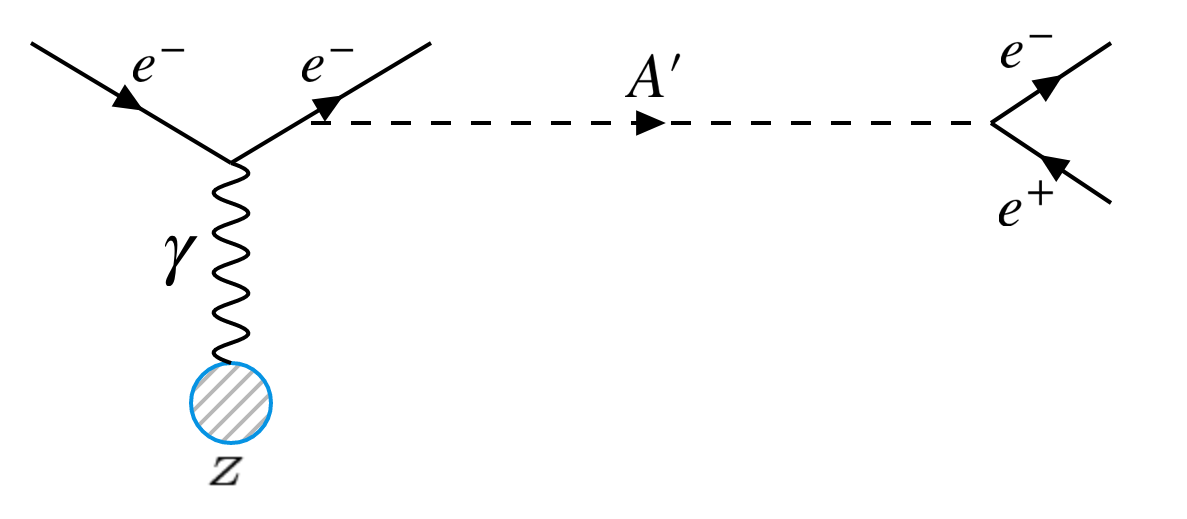
\includegraphics[width=14.5cm]{thesis_figures/VISIBLE.png}
\caption{Visible mode }
\label{fig:Visible_feynman}
\end{figure}

\begin{figure}[t!]
\centering
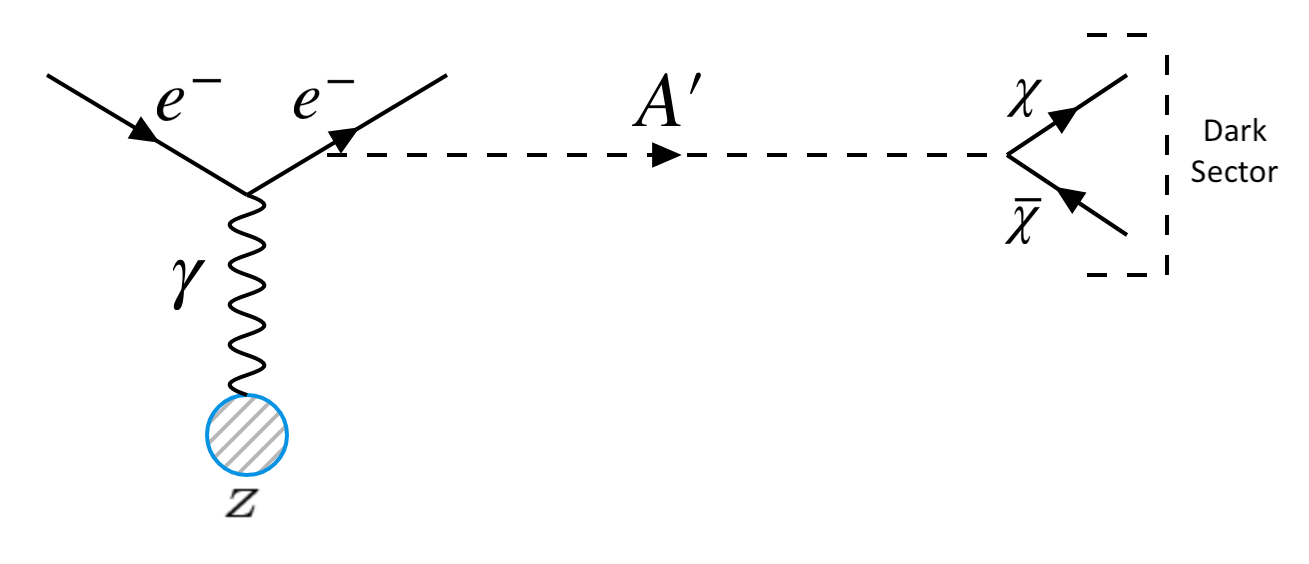
\includegraphics[width=15cm]{thesis_figures/INVISIBLE.png}
\caption{Invisible mode }
\label{fig:Invisible_feynman}
\end{figure}

The production and detection mechanisms discussed offer us the basic ingredients needed to set up an experiment for the detection of $A'$. One of the simpler layouts for such an experiment is an electron beam dump experiment. NA64 falls in this category, the setup of which is discussed in the next chapter.
\begin{figure}[t!]
\centering
  \begin{minipage}[t]{.45\textwidth}
    \centering
    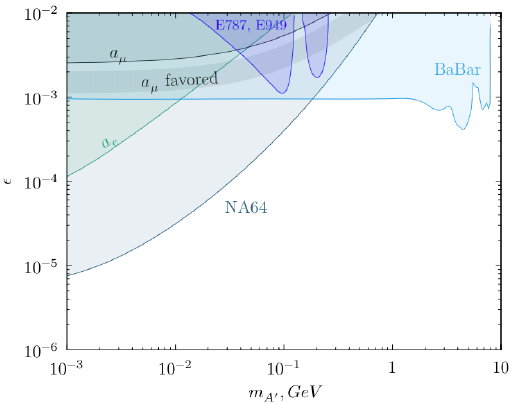
\includegraphics[width=\textwidth]{thesis_figures/exclusion_invisible.png}
    \caption{Current limits for invisible mode for 90\% C.L. exclusion region in the ($m_{A'},\epsilon$) plane ~\cite{}.}
    \label{fig:exclusion_invisible}
  \end{minipage}
  \hfill
  \begin{minipage}[t]{.45\textwidth}
    \centering
    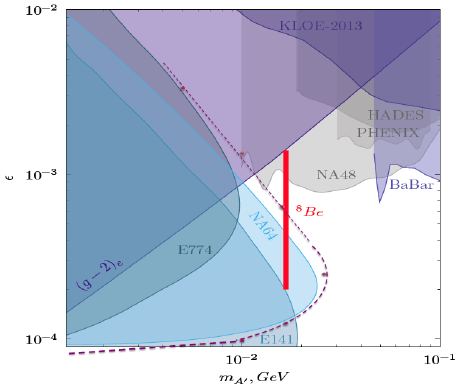
\includegraphics[width=\linewidth]{thesis_figures/exclusion_visible_latest.png}
    \caption{Current limits for invisible mode for 90\% C.L. exclusion region in the ($m_{A'},\epsilon$) plane. The blue plane is with 2017 data and the dotted line is with 2017+2018 data for NA64. The red line is the region that might explain the X17 boson~\cite{}.}
    \label{fig:exclusion_visible}
  \end{minipage}
\end{figure}


%%% Local Variables:
%%% mode: latex
%%% TeX-master: "mythesis"
%%% End:
